
\chapter{Background}
\label{chap:background}
The present chapter covers background information referred to throughout the thesis. A brief introduction to the \textit{Reinforcement Learning Problem} is first given in \RefSec{sec:rl}. Two Single-agent Markov Decision Process frameworks are then introduced in \RefSec{sec:sarl}. The time complexity of exact solutions to these problems is analyzed in \RefSec{sec:intract}. An overview of several exact and approximate solving techniques is given in \RefSec{sec:stateart}. Finally, \RefSec{sec:repstat} briefly discusses \textit{first-order} representations of Markov Decision Processes.
\section{The Reinforcement Learning Problem}
\label{sec:rl}
Reinforcement Learning (RL) is a Machine Learning paradigm, in which a learning entity, typically called agent, learns in an environment by performing actions and observing the environment's response \cite{RLgeneral}. More specifically, when an agent performs action $a_t$ at time $t$, the environment, initially in state $s_t$, returns its new state $s_{t+1}$ as well as a reward $r_{t+1}$ to the agent. The agent aims to maximize the reward it can accumulate over time. The general feedback loop is schematized in \RefFig{fig:feedback}.

\begin{figure}[h]
  \begin{center}
    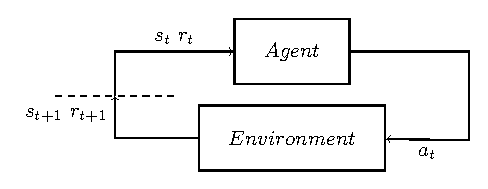
\includegraphics{images/MasterThesisRLLoop.pdf}
  \end{center}
  \caption{Reinforcement Learning feedback loop}\label{fig:feedback}
\end{figure}

The RL paradigm can be formalized in Single-agent and Multi-agent settings. Several properties emerging from the former no longer hold in the latter. The fundamental single-agent formalisms are now covered in further detail.

\section{Single-agent formalisms}
\label{sec:sarl}
This section formalizes the fundamental concepts of learning in single-agent settings. In the present thesis, the following properties of the environment are assumed to be true:
\begin{itemize}
    \item The environment behaves stochastically, meaning that given a starting state and an action performed, the environment is not guaranteed to transition to the same new state each time. A robot expected to jump forward one meter might, for instance, miss the target and jump too far.
    \item The environment is stationary, meaning that the transition rules which the environment abides by do not change over time. 
    \item The environment obeys the \textit{Markov property}. This property states that the probability of the environment transitioning to any given state is solely conditioned by the current state of the environment and the current action of the agent \cite{Russell:2009:AIM:1671238}.
    \item The state space is discrete and comprised of a finite number of elements. 
\end{itemize}
\RefSec{sec:mdp} covers the simplest form of Markov Decision Processes. \RefSec{sec:pomdp} then introduces a common extension to the initial framework.

\subsection{Fully Observable Markov Decision Processes}
\label{sec:mdp}
The Single-Agent Learning (SAL) problem can be formally modeled as a Markov Decision Process.
\begin{definition}[Fully Observable MDP]
\label{def:fomdp}
A fully observable Markov Decision Process, or simply MDP, $\mathcal{M}$ is formally defined as a tuple \cite{Russell:2009:AIM:1671238}
\begin{align*}
    \mathcal{M} := \big \langle \mathcal{S}, \mathcal{A}, \mathcal{T}, \mathcal{R} \big \rangle
  \end{align*}
where:
\begin{itemize}
    \item $\mathcal{S}$ is the set of possible states of the environment.
    \item $\mathcal{A}$ is the set of possible actions.
    \item $\mathcal{T} : \mathcal{S} \times \mathcal{A} \times \mathcal{S} \rightarrow [0,1]$ is called the \textit{transition model}. $\mathcal{T}(s,a,s')$ returns the probability of the environment transitioning from state $s$ to state $s'$ after action $a$ is performed.
    \item $\mathcal{R}: \mathcal{S} \times \mathcal{A} \rightarrow \R$ is called the \textit{reward function}. $\mathcal{R}(s,a)$ returns the immediate reward received after performing action $a$ in state $s$.
\end{itemize}
\end{definition}
The objective of an MDP agent is to maximize its long-term cumulative reward, called \textit{utility}. While the utility can be defined in several ways, the most commonly used definition is called \textit{discounted future reward}. The utility $U$ of a \textit{finite} state-action sequence, sometimes called \textit{episode}, $E = \big \langle s_0,a_0,s_1, a_1,..., s_T, a_T \big \rangle$ is defined as \cite{Nitti2017}:
\begin{align}
\label{eq:utility}
    U(E) = \sum_{t=0}^{T} \gamma^t \mathcal{R}(s_t, a_t)
\end{align}
where $\gamma \in [0,1]$ is called the \textit{discount factor}. An agent moves about in the environment by following a \textit{policy}.

\begin{definition}[Finite-horizon policy]
\label{def:policymdp}
A finite-horizon policy $\pi : \mathcal{S} \times \N \rightarrow \mathcal{A}$ is a function that maps each environment state and remaining time-steps to the action the agent should take.
\end{definition}
The \textit{expected utility}, or \textit{value}, of being in any state $s_t$ at time-step $t$, while following policy $\pi$, with $d$ time-steps remaining, is defined as \cite{Nitti2017}:
\begin{align}
    V^{\pi}(s_t, d) = \E[U(E_t) \, | \, s_t, \pi] = \E \big[ \sum_{k = t }^{t+d} \gamma^{k-t} \mathcal{R}(s_k, a_k) \, \big| \, s_t, \pi \big ]
\end{align}
where $E_t$ is the sub-sequence of $E$ starting at time-step $t$. An optimal policy $\pi^\star$ is a policy such that
\begin{align}
    \forall s \in \mathcal{S}, \forall d \in \N, \forall \pi : V^{\star}(s,d) \geq V^{\pi}(s,d) 
\end{align}
where $V^{\star} : \mathcal{S} \times \N \rightarrow \R$ is the value function associated with optimal policy $\pi^{\star}$.
This policy satisfies the \textit{optimality equations}, also known as the \textit{Bellman equations}:
\begin{align}
\label{eq:bellman}
        \begin{dcases}
            V^{\star}(s, d) := \max_{a \in \mathcal{A}} \Big\{ \mathcal{R}(s,a) + \gamma \sum_{s' \in \mathcal{S}} \mathcal{T}(s,a,s') V^{\star}(s', d-1) \Big\}  &\forall s \in \mathcal{S}, d > 1
            \\
            V^{\star}(s, 1) := \max_{a \in \mathcal{A}} \Big\{ \mathcal{R}(s,a) \Big\} &\forall s \in \mathcal{S}
        \end{dcases}
    \end{align}
    
MDPs are adequate for modeling a range of stochastic domains in which the state of the environment is fully observable at all times. Yet, fully observable environments can not always be taken for granted. The problem of partial observability is covered hereafter.

\subsection{Partially Observable Markov Decision Processes}
\label{sec:pomdp}
Alongside the stochastic nature of many environments, a prevalent form of uncertainty lies in the partial observability of several domains. Take a robot equipped with proximity sensors advancing in a room filled with obstacles. This robot does not sense the actual state of the room. Rather, it can only sense what the sensors pick up, and may very well bump into obstacles that were missed during the sensing process. Partially Observable Markov Decision Processes are an extension of classic MDPs that deal with the problem of partial observability \cite{Russell:2009:AIM:1671238}.
\begin{definition}[Partially Observable MDP]
A partially observable MDP, or POMDP, $\mathcal{P}$ is formally defined as a tuple
\begin{align*}
    \mathcal{P} := \big \langle \mathcal{S}, \mathcal{A}, \mathcal{T}, \mathcal{R}, \Omega, \mathcal{O} \big \rangle
  \end{align*}
where:
\begin{itemize}
    \item $\mathcal{S}$, $\mathcal{A}$, $\mathcal{T}$ and $\mathcal{R}$ are defined as in \RefDef{def:fomdp}.
    \item $\Omega$ is the set of observations.
    \item $\mathcal{O} : \mathcal{A} \times \mathcal{S} \times \Omega \rightarrow [0,1]$ is called the \textit{observation function} or \textit{sensor model}. $\mathcal{O}(a,s',o)$ returns the probability of making observation $o$ after performing action $a$ and the environment transitioning to state $s'$.
\end{itemize}
\end{definition}
Instead of working with the actual states of the environment, the POMDP framework introduces the notion of \textit{belief states}.
\begin{definition}[Belief state]
A belief state $b \in \Delta(\mathcal{S})$ is a probability distribution over the possible states of the environment. As such, $b(s)$ returns the probability of being in state $s$. Furthermore,
\begin{align*}
    \sum_{s \in \mathcal{S}} b(s) = 1
\end{align*}
\end{definition}
Suppose the agent makes observation $o$ after taking action $a$ in current belief state $b$. The updated belief state $b'$ is computed using the \textit{state estimation function} $SE$ defined as follows:
\begin{align}
\label{eq:belief}
    b' := SE(b,a,o) := \Big\{(s',p) \,\,\Big| \,\,s' \in \mathcal{S} \land p =  \frac{\mathcal{O}(a,s',o) \sum_{s} \mathcal{T}(s,a,s') b(s)}
    {P(o | b, a)} \Big\}
\end{align}
where $P(o | b,a) = \sum_{s' \in \mathcal{S}} \mathcal{O}(a,s',o) \sum_{s \in \mathcal{S}} \mathcal{T}(s,a,s') b(s)$ is a normalizing constant.
The optimal value function $V^{\star} : \Delta(\mathcal{S}) \times \N \rightarrow \R$ satisfies the following \textit{optimality equations} (\forall b \in \Delta(\mathcal{S})):

\begin{align}
        \begin{dcases}
            V^{\star}(b, d) := \max_{a \in \mathcal{A}} \Big\{ \sum_{s \in \mathcal{S}}\mathcal{R}(s,a) b(s) + \gamma \sum_{o \in \Omega} P(o | b,a) V^{\star}(SE(b,a,o), d-1) \Big\}  
            \\
            V^{\star}(b, 1) := \max_{a \in \mathcal{A}} \Big\{ \sum_{s \in \mathcal{S}}\mathcal{R}(s,a) b(s) \Big\} 
        \end{dcases}
    \end{align}


\section{Time complexity of solving Markov Decision Processes via Value Iteration}
\label{sec:intract}
The present section covers the time complexity of a solving strategy for fully and partially observable MDPs called the value iteration algorithm. Partial observability is shown to render the computation of exact solutions intractable, even in single-agent settings.

Value iteration (VI) is an iterative process that considers successively longer planning horizons to produce exact, i.e. optimal, solutions to fully and partially observable MDPs \cite{phdthesispomdp}. This is accomplished by computing the $i$-th horizon optimal value function at each iteration $i$, using the $i-1$-th horizon optimal value function computed at the previous iteration. The termination criterion is different for infinite- and finite-horizon problems: in infinite horizon problems, termination is reached when the value function converges, i.e., when it no longer changes sufficiently between two iterations. The final value function is then kept. In finite-horizon problems, termination is reached when the value function has been computed for each step within the horizon depth. The value functions produced at each step are all kept. The fully observable MDP VI algorithm was introduced by \textit{Bellman} in 1957 \cite{Bellman:1957}, while \textit{Sondik} developed its counterpart for partially observable environments in the early 1970s \cite{sondik1973}.
\subsection{VI for fully observable, finite-horizon MDPs}
Let $\mathcal{M}$ be a finite horizon MDP of horizon $d$, $|\mathcal{S}|$ the number of states, and $|\mathcal{A}|$ the number of actions of $\mathcal{M}$. Each iteration $i$ of the VI planning algorithm computes the optimal value $V^{\star}(s,i)$ for each state $s$, i.e. $|\mathcal{S}|$ computations in total. Each such computation involves the maximization over $|\mathcal{A}|$ actions. For each action $a$, the evaluation involves the summation over $|\mathcal{S}|$ states. The time complexity of the VI algorithm is thus \cite{mdpcomp}
\begin{align}
    \mathcal{O}(d |\mathcal{S}|^2|\mathcal{A}|).
\end{align}
The algorithm is given in \RefAlg{alg:valitmdp}.

\begin{algorithm}[H]
\caption{Value iteration for finite-horizon MDPs}\label{alg:valitmdp}
\begin{algorithmic}[1]
\Procedure{Value-Iteration}{}
    
\For {$i = 1 \rightarrow d$}
    \ForAll{$s \in \mathcal{S}$} 
        \If {$i == 1$} \State $V^{\star}(s, 1) \leftarrow \max_{a \in \mathcal{A}} \Big\{ \mathcal{R}(s,a) \Big\}$
         \Else \State $V^{\star}(s, i) \leftarrow \max_{a \in A} \Big\{ \mathcal{R}(s,a) + \gamma \sum_{s' \in S} \mathcal{T}(s,a,s') V^{\star}(s', i-1) \Big\}$
        \EndIf
    \EndFor
\EndFor

\EndProcedure
\end{algorithmic}
\end{algorithm}
As such, MDP VI is polynomial in the number of states $|\mathcal{S}|$. The algorithm is said to be \textit{tractable} and belongs to complexity-class \textbf{P}.
\subsection{VI for partially observable, finite-horizon MDPs}
VI is less straightforward with POMDPs than with fully observable MDPs. This comes as a direct result of the belief space being continuous, making it impossible to compute $V^{\star}(b,n)$ for each belief state $b$ the way it is done for fully observable MDPs \cite{Russell:2009:AIM:1671238}. \\ The optimal value function $V^{\star}$ turns out to always be \textit{piecewise linear} and \textit{convex} in the belief space \cite{RePEc:inm:oropre:v:21:y:1973:i:5:p:1071-1088}. Formally, this equates to $V^{\star}$ having the following form:
\begin{align}
    V^{\star}(b, n) = \max_{\alpha \in \mathcal{V}_n} \sum_{s \in \mathcal{S}}\alpha(s) b(s) = \max_{\alpha \in \mathcal{V}_n} \alpha \cdot b
\end{align}
where $\mathcal{V}_n = \{\alpha_0,\alpha_1,...,\alpha_m \}$ is a set of $\alpha$-vectors, each $\alpha$-vector maintaining the parameters of an $|\mathcal{S}|$-dimensional hyperplane describing the optimal value function over a region of the belief space \cite{Pineau-2003-8730}. In other words, $V^{\star}$ is the upper surface of the collection of hyperplanes described by the $\alpha$-vectors \cite{uppersurface}. Each $\alpha$-vector is associated with a specific conditional plan, that is, the region over which one hyperplane in $\mathcal{V}_n$ dominates all other hyperplanes in $\mathcal{V}_n$ is associated with one optimal action. Each iteration $i$ of the algorithm  consists of two steps \cite{phdthesispomdp}:
\begin{itemize}
    \item Generation of potentially useful $i$-th horizon $\alpha$-vectors. This step first consists of the generation of $\mathcal{O}(|A||\Omega||\mathcal{V}_{i-1}|)$  projections in total. The algorithm then proceeds to compute $\mathcal{O}(|A||\mathcal{V}_{i-1}|^{|\Omega|})$ cross-sums. Each $\alpha$-vector is computed in $\mathcal{O}(|S|^2)$ time \cite{Pineau-2003-8730,hauskrecht,crosssum}. The generation step thus has a worst-case complexity 
    \begin{align}
        \mathcal{O}(|S|^2|A||\mathcal{V}_{i-1}|^{|\Omega|})
    \end{align}
    \item Pruning of fully-dominated $\alpha$-vectors. This step usually involves the solving of a linear program and does not add to the asymptotic complexity of the algorithm \cite{KAELBLING199899}.
\end{itemize}
The corresponding algorithm is given in \RefAlg{alg:valitpo}. Solving POMDP via VI is exponential in $|\Omega|$ and, as such, is said to be \textit{intractable}. While the notion of \textit{intractability} will be formalized in \RefChap{chap:related}, it is worth noting at this point that the \textit{intractability} of this single-agent-based algorithm is evocative of the challenges encountered in most multi-agent learning settings.

\begin{algorithm}[H]
\caption{Value iteration for finite-horizon POMDPs}\label{alg:valitpo}
\begin{algorithmic}[1]
\Procedure{Value-Iteration}{}


\ForAll{$a \in \mathcal{A}$} 
    \State $\mathcal{V}_1^{-} \leftarrow \alpha^{a,*}(s) = {R}(s,a)$
\EndFor
    
\For {$i = 2 \rightarrow d$}
    \ForAll{$a \in \mathcal{A}$} 
        \State $\mathcal{V}_i^{a,*} \leftarrow \alpha^{a,*}(s) = \mathcal{R}(s,a)$
            \ForAll{$o \in \Omega$} 
                \ForAll{$\alpha_{j} \in \mathcal{V}_{i-1}^{-}$} 
                    \State $\mathcal{V}_i^{a,o} \leftarrow \alpha_j^{a,o}(s) = \gamma \sum_{s' \in \mathcal{S}} \mathcal{T}(s,a,s') \mathcal{O}(a,s',o) \alpha_{j}(s')$
                \EndFor
            \EndFor
        \EndFor
        \ForAll{$a \in \mathcal{A}$}
            \State $\mathcal{V}_i^{a} = \mathcal{V}_i^{a,*} \oplus \mathcal{V}_i^{a,o_1} \oplus ... \oplus \mathcal{V}_i^{a,o_{|\Omega|}}$
        \EndFor
        \State $\mathcal{V}_i = \bigcup_{a \in \mathcal{A}} \mathcal{V}_i^a$
        \State $\mathcal{V}_i^{-} = \text{PRUNE}(\mathcal{V}_i)$
    \EndFor
\EndProcedure
\end{algorithmic}
\end{algorithm}
%As such, in accordance with equation (\ref{eq:intract}), POMDP VI is \textit{intractible}, regardless of the pruning strategy used \cite{intractt}.
\section{Model-based solving techniques}
\label{sec:stateart}
Various algorithms have followed since the introduction of VI. The present section first provides an overview of the different algorithm classes, after which several solving techniques are described in further detail.
\subsection{Online and offline learning algorithms}
\label{sec:onlineoffline}
The single-agent (and later multi-agent) frameworks, and more specifically learning algorithms, considered in this thesis can be divided into two categories:
\begin{itemize}
    \item \textit{Offline learning algorithms}: A learning algorithm is said to be offline if the learning phase takes place entirely prior to the execution of the policy. By the end of the learning phase, a course of action, optimal or not, is known for every possible happening, i.e., state and horizon, and the policy no longer changes during the execution \cite{offlineonline}. Offline algorithms are sometimes referred to as traditional search in the literature. %Offline learning furthermore assumes knowledge of the \textit{rules} of the environment, i.e. the \textit{transition model}, as well as of the \textit{reward scheme}.
    \item \textit{Online learning algorithms}: A learning algorithm is said to be online if learning and execution are interleaved, and planning during the learning phase is done using information leveraged during the execution. This often reduces the sum of planning and execution cost, but has the drawback of leading to incomplete policies, as the best course of action is only computed for the information available. Online algorithms are sometimes referred to as agent-centered search \cite{Koenig_2001}. %and do not require knowledge of the environment dynamics, although some do.
\end{itemize}
\subsection{Exact offline methods}
In 1960, shortly after Bellman's introduction of the VI algorithm, \textit{Howard} developed an alternative to MDP VI called \textit{policy iteration} \cite{howard:1960}. This algorithm proved to have faster convergence properties, but, due to its mathematical formulation, involving the solving of a system of linear equations is usually used with smaller state spaces \cite{policyadv}. In 1963, \textit{d'Epenoux} showed that the Bellman equations could be rewritten as an equivalent linear program \cite{linprog}.
While these methods are used to produce exact optimal solutions, they suffer from the \textit{curse of dimensionality}. In fact, as the number of state variables grows, it becomes increasingly computationally expensive to compute exact policies, as they need to be computed over the entire state space. The problem is even more alarming with POMDPs, due to their associated intractability. As such, in a problem with $|\mathcal{S}|$ states, a POMDP solver has to operate in a $(|\mathcal{S}|-1)$-dimensional and continuous belief space \cite{Pineau-2003-8730}.

\subsection{Approximate methods}
Approximate MDP and POMDP solving methods were introduced to counter the unscalability inherently associated with the exact methods. To accomplish the alleviation of complexity, several distinct strategies can be identified\footnote{Note that the algorithms presented hereafter do not form an exhaustive list by any means.}:
\begin{itemize}
    \item \textit{Offline} approximations: Several \textit{point-based} approximations have been proposed in the literature. Notably, in 1991, \textit{Lovejoy} employed a grid-based approximation of the POMDP belief-space, to then produce lower and upper value function bounds, using interpolation \cite{Lovejoy1991ComputationallyFB}. Later, \textit{Poon} proposed a grid-based algorithm that computes the gradient alongside the value at each grid point, in an attempt to make the algorithm more generalizable to unexplored belief points, due to the \textit{piecewise linear} and \textit{convex} nature of the exact optimal solution \cite{Poon2001AFH}. In 2003, \textit{Pineau et al.} introduced \textit{point-based value iteration} (PBVI) for POMDPs \cite{Pineau-2003-8730}, building on top of Poon's work. The novelty in this approach lies in the careful selection of belief points to apply value iteration and gradient updates to. The belief points are selected using \textit{stochastic trajectories}. In short, given a current belief-set $\mathcal{B}$, containing the belief points currently considered for value iteration, a new belief point $b$ is added to $\mathcal{B}$ if it is directly reachable from $\mathcal{B}$ and would improve the uniformity of the density of $\mathcal{B}$ in the set of reachable belief points the most, i.e., $b$ is the furthest away from any point in $\mathcal{B}$. A number of methods have built on top of PBVI since, including HSVI (Smith $\&$ Simmons, 2004) \cite{hsvi} and Perseus (Spaan $\&$ Vlassis, 2005) \cite{perseus}.
    \item \textit{Online} approximations: Initial research on approximate online methods was the result of two issues inherently associated with offline approaches: firstly, the time it takes an offline algorithm to solve a (PO)MDP increases rapidly with the number of possible situations, even when carefully selecting the (belief) states to perform calculations on. Secondly, if the transition model used to compute the policy were to change during the execution of the policy, said policy would have to be recomputed from scratch \cite{offlineonline}. 
    
    The general framework for model-based online planning for MDPs can be described as the interleaving of two phases, the \textit{planning phase}, and the \textit{execution phase}. 
    \begin{itemize}
        \item The planning phase consists of the solving of a state-space search problem. This problem is characterized by the MDP set of states $\mathcal{S}$, its set of actions responsible for the state transitions $\mathcal{A}$, an initial state $s_0 \in \mathcal{S}$, and the value function $V$ giving the value of state transitions \cite{searchheur}. Given the current state of the environment $s_0$, an AND/OR tree of depth $D$, specified beforehand, is first constructed. The OR-nodes are state-nodes, while the AND-nodes are action-nodes. The best value is then propagated back to the root of the tree, starting at the leaves and using the Bellman equations (Equation \ref{eq:bellman}). More specifically, assuming the leaves of the search tree are not terminal nodes, a starting \textit{heuristic} estimate $h$ of the true value defined as 
        \begin{align}
            h: \mathcal{S} \rightarrow \R
        \end{align}
        such that $h(s) \leq V(s) \,\, \forall s \in \mathcal{S}$ (\textit{admissibility} of a heuristic, the estimate of the value must always underestimate the true value \cite{Russell:2009:AIM:1671238}) is required. The most straightforward heuristic is the base case of the Bellman equations, as it does not take into account the recursive call of the value function to itself. The action nodes then compute the \textit{state-action} value using the heuristic values computed at the state nodes right below (children). Non-leaf state nodes then use the maximum of the state-action values of their children as their value. Finally, at the root of the tree, the child action associated with the highest state-action value is returned. \RefFig{fig:tree} illustrates a look-ahead search of depth $D = 1$.
        \begin{figure}[h]
    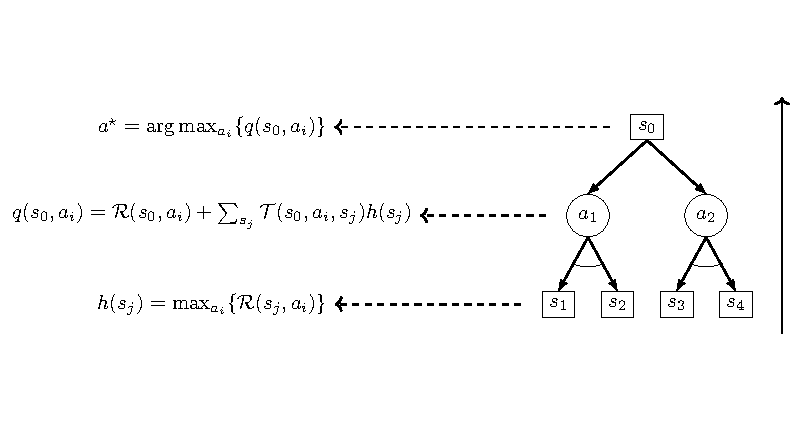
\includegraphics[width=0.9\textwidth]{images/MasterThesisAndOrTree(1).pdf}
  \caption{Look-ahead search space, depth $D = 1$ (MDP)}
  \label{fig:tree}
\end{figure}
\item The execution phase consists in executing the action, say $a^{\star}$, associated with the highest value estimate. The environment returns a new state $s'$ that may now be used as the root of the search tree during the following planning phase.
    \end{itemize}
    
    \item \textit{Hybrid Offline-Online} approximations: In 2006, \textit{Parquet et al.} \cite{articlepomh} propose three algorithms for POMDPs that combine the advantages of several \textit{online} (RTBSS \cite{rtbss}, RTDP-BEL \cite{rtdpbel}) and \textit{offline} algorithms ($Q_{MDP}$ \cite{qmdp}, PBVI \cite{Pineau-2003-8730}), and show that they can often outperform \textit{online} and \textit{offline} approaches alone. In 2011, \textit{Maniloff et al.} \cite{maniloff} introduce \textit{Hybrid Value Iteration} for POMDPs, an algorithm that combines PBVI and look-ahead (tree) search to meet real-time constraints. The heuristic tree search is thereby used to occasionally make improvements to the value function initially computed offline using PBVI.
\end{itemize}


\section{Relational representation of the state space}
\label{sec:repstat}
Thus far, states have been handled like elements with no apparent relations between them. Concretely, the state spaces were not described in terms of a set of features that apply to and make up its elements. Consequently, as the environments described become more complex and are made up of more features, the state spaces grow exponentially with the number of features \cite{masbook}, thus quickly leading to unmanageable transition models. It is worth briefly discussing ongoing research in the field of \textit{relational} decision-making.


Many real-world domains are inherently relational \cite{Nitti2017}. In particular, from a \textit{logic programming} point of view, the state space of an environment can be described by a collection of \textit{relations} that jointly make up the features of the state space \cite{bout2, rrmdp}, and the states are \textit{Herbrand interpretations} of said collection \cite{relationallogic}. As such, an environment that describes a blocks world could be made up of the relations \texttt{on/2} and \texttt{clean/1}, while a possible world, that is, a state could be \texttt{on(A,C)}, \texttt{clean(B)}, where \texttt{A}, \texttt{B}, and \texttt{C} represent blocks (the example is taken from \textit{Nitti et al.}, 2017 \cite{Nitti2017}). This state is schematized in \RefFig{fig:block}. Actions are then described as facts (e.g., \texttt{move(A,B)}), and the state transition model is modeled through probabilistic rules. In 2001, \textit{Boutilier et al.} \cite{bout2} introduced the first \textit{relational} (\textit{first-order}) MDP (RMDP) and provided an algorithm for solving RMDPs using the \textit{Bellman equations} called \textit{Symbolic Dynamic Programming}. This \textit{structured} approach to the representation of states makes it possible to solve complex (real-world) problems of relational nature, that is, problems in which states are made up of multiple features.




\begin{figure}[h]
\centering
    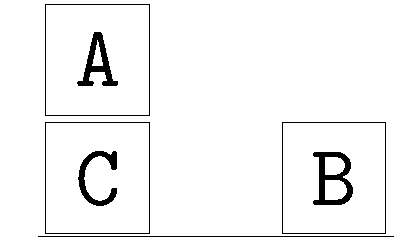
\includegraphics[width=0.25\textwidth]{images/MasterThesisRelationalDraw.pdf}
  \caption{A state of the blocks world}
  \label{fig:block}
\end{figure}


Note that, due to the simple nature of the scenarios discussed in later chapters, and given that the use of this representation is not indispensable to the study of the framework of interest of this thesis, we do not adopt a \textit{relational} approach for representing the states of the environment.